\documentclass[letterpaper]{article} % DO NOT CHANGE THIS
% W3PHIAI uses single-blind review, so authors are shown (AAAI-27 Author Kit).
\usepackage{aaai2027}  % DO NOT CHANGE THIS
\usepackage[hyphens]{url}  % DO NOT CHANGE THIS
\usepackage{graphicx} % DO NOT CHANGE THIS
\urlstyle{rm} % DO NOT CHANGE THIS
\def\UrlFont{\rm}  % DO NOT CHANGE THIS
\usepackage{natbib}  % DO NOT CHANGE THIS AND DO NOT ADD ANY OPTIONS TO IT
\usepackage{caption} % DO NOT CHANGE THIS AND DO NOT ADD ANY OPTIONS TO IT
\frenchspacing  % DO NOT CHANGE THIS
\usepackage{booktabs}
\usepackage{amsmath}
\usepackage{array}
\newcommand{\lbl}{\textsc{Label}}
\pdfinfo{
/TemplateVersion (2027.1)
}
\nocopyright % workshop paper, not AAAI proceedings: no AAAI copyright slug
\setcounter{secnumdepth}{2}

\title{\lbl{}: Literature Asymmetry between Efficacy and Limits\\in Drug Knowledge and Language Models}
\author{
    S M Rayeed,
    Chuck Stewart,
    Yao Ma
}
\affiliations{
    Rensselaer Polytechnic Institute, Troy, NY, USA
}

\begin{document}

\maketitle

\begin{abstract}
Every drug carries two kinds of fact: its efficacy, what it treats, and its
limits, who must not take it. The limits protect patients, yet we find they are
what prose writes down least. We measure, on the same facts, how often text names a drug's
indications and contraindications and how often a language model knows them.
Comparing each drug against itself on 574 drugs from PrimeKG, the odds that a
benefit fact is named are 2.43 times those of a safety fact in Wikipedia, 2.77
times in PubMed abstracts, and 2.19 times in the two combined (95\% CI
1.86--2.57). We call this the \lbl{} asymmetry (literature asymmetry between
efficacy and limits). It disappears in the FDA drug label, scored with the same
matcher on the same edges (odds ratio 1.05, 95\% CI 0.88--1.25): safety facts
are recorded where regulation requires them and left out of the prose.
Models show the prose pattern. Across Qwen2.5 from 0.5B to 14B parameters,
indication accuracy rises 18 points while contraindication accuracy stays
within 7 points of chance at every size, and the gap reappears in four models
from three families under harder distractors. Giving the model the drug's page
helps safety facts about as much as benefit facts when the page names them
($+14.2$ against $+11.1$ points; difference $-3.1$, 95\% CI $-11.6$ to $+5.1$),
consistent with a documentation bottleneck rather than a reading failure. A control graph whose two relations both describe benefit shows no gap
once each drug's number of edges is held fixed. Medication-safety questions
should therefore be routed to the label and to structured drug databases rather
than to text alone.
\end{abstract}

\section{Introduction}

Look up a medicine and the page will tell you what it treats. It is far less
likely to tell you who must never take it. A drug's indications (``metformin
treats type 2 diabetes'') and its contraindications (``ciprofloxacin should not
be given to people with myasthenia gravis'') are both recorded in structured
drug databases such as DrugCentral \citep{ursu2017drugcentral}. In free text,
the two are not recorded equally.

This matters because language models learn from free text, and people now ask
them about their medications. If the safety relation is the one text
documents least, then the question with the highest cost of error is the one a
model is least prepared to answer. It also locates the failure before the
model. A model that misses a contraindication is not necessarily ignoring
safety; the fact may never have been written where it could learn it. That
changes the remedy. Better prompting and better retrieval over prose are unlikely to surface a
fact that was never written down there, while a structured source can.

Two literatures touch this question without joining it. Pharmacy and
informatics studies audit reference text, typically a small set of drugs
compared against a textbook \citep{clauson2008scope,kraenbring2014accuracy}.
Model benchmarks built from drug knowledge graphs score what models answer
\citep{liu2026mhgraphbench}, but do not trace errors to the text. Neither
measures text and models on the same facts, and neither controls for the
obvious confound: famous drugs have long articles and many papers.

We join the two measurements on the same facts and compare each drug against
itself (Figure~\ref{fig:pipeline}). Our contributions are:
\begin{itemize}
\item A within-drug design over 574 PrimeKG drugs that compares the
documentation of each drug's indications with its contraindications, so that
article length, popularity, and research attention cancel.
\item Three corpora with different authors and purposes: English Wikipedia,
PubMed abstracts with a separate retrieval budget for each relation, and the
FDA drug label. Prose shows the gap; the label, on the same edges, does not.
\item A model-side probe on 1,800 facts across five sizes of one model family,
a paired test of whether scale helps the two relations equally, and a
replication under harder distractors in four models from three families.
\item A retrieval test that gives the model the drug's page, separated by
whether the page names the fact, which shows that retrieval helps safety facts
fully when they are written down.
\item A negative control on Hetionet, whose two drug--disease relations both
describe benefit, and a routing design for clinical agents that follows from
the measurements.
\end{itemize}

The finding, which we call the \lbl{} asymmetry, is simple: prose names a
drug's efficacy about twice as often as its limits, the regulatory label does
not, and models follow the prose.

\section{Related Work}

\paragraph{Drug information in reference text.}
Wikipedia is among the most consulted health resources on the web
\citep{heilman2011wikipedia}, and its drug articles have been audited several
times. \citet{clauson2008scope} compared Wikipedia with a professional drug
compendium and found it less complete, with frequent omissions.
\citet{kraenbring2014accuracy} compared 100 drug articles with pharmacology
textbooks and found high accuracy but incomplete coverage. These audits
establish that coverage is uneven. They cover about a hundred teaching drugs,
they grade text against a textbook rather than against a drug's full set of
relations, and they do not connect coverage to what models learn.

\paragraph{Structured drug knowledge.}
Drug safety is recorded in resources built for that purpose. DrugCentral
curates indications and contraindications from drug labels
\citep{ursu2017drugcentral}, SIDER extracts side effects from package inserts
\citep{kuhn2016sider}, and openFDA exposes the full text of FDA structured
product labels \citep{kasshout2016openfda}. Knowledge graphs such as PrimeKG
and Hetionet integrate these sources with disease ontologies
\citep{chandak2023primekg,himmelstein2017hetionet}. These resources make it
possible to ask, fact by fact, whether the same information also appears in
free text.

\paragraph{Medical knowledge in language models.}
Large language models answer medical licensing questions well
\citep{singhal2023clinical,singhal2025expert}, but benchmarks built from
knowledge graphs show uneven knowledge across relation types. MHGraphBench
\citep{liu2026mhgraphbench} probes models with questions generated from PrimeKG
and reports that relation prediction is much harder than entity typing. These
benchmarks describe what models get wrong; they do not trace the error to the
text the models learned from.

\paragraph{Corpus frequency and model knowledge.}
A separate line of work links what models know to how often facts appear in
pretraining data. \citet{kandpal2023longtail} show that question-answering
accuracy rises with the number of documents relevant to a question, and
\citet{mallen2023trust} show that models fail on less popular entities, where
retrieval helps most. LMEnt \citep{gottesman2026lment} annotates entity
mentions in a pretraining corpus to trace knowledge to its sources. These
studies measure entities or questions. Two facts about the same drug receive
the same popularity score, so they cannot distinguish a drug whose benefits are
written down from one whose risks are. Our measurement is per fact and
compares relations within a drug.

\paragraph{Retrieval as a remedy.}
Retrieval-augmented generation \citep{lewis2020rag} is the standard answer to
missing parametric knowledge: give the model a relevant document. In medicine,
the MIRAGE benchmark \citep{xiong2024medrag} shows that retrieval from PubMed,
textbooks, and Wikipedia improves question answering, with gains that depend
on the corpus and the retriever. These evaluations report accuracy per
question set, not per relation, and do not ask whether the retrieved text
contains safety facts at the rate it contains benefit facts. Work on
sufficient context \citep{joren2025sufficient} shows that the benefit depends
on whether the retrieved text actually contains the answer. Our results
measure that condition for drug safety and show that it fails far more often
for contraindications than for indications, in every prose corpus we tested.
\citet{bang2025contraindications} answer contraindication questions from a
drug utilization review database, the routing our measurements support.

\begin{figure*}[t]
\centering
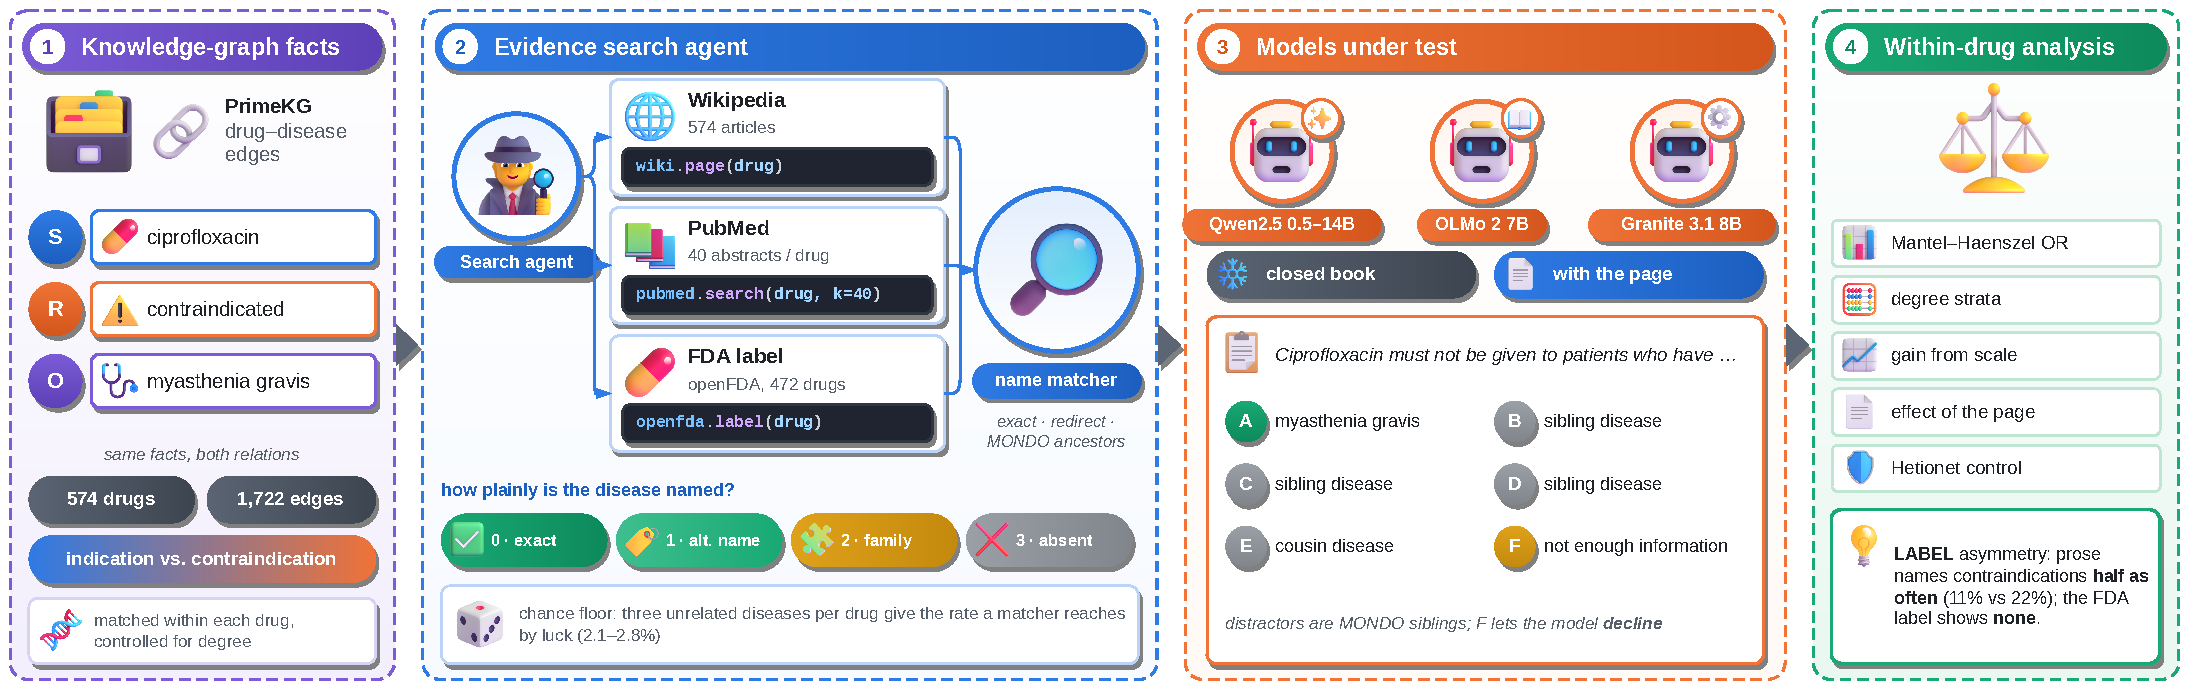
\includegraphics[width=\textwidth]{fig_pipeline.pdf}
\caption{Study design as an agent pipeline. (1) PrimeKG supplies both relations
for the same drugs; (2) a search agent retrieves Wikipedia, PubMed and FDA label
text, and a name matcher scores how plainly each names the disease; (3) the
models under test answer the same facts closed book and with the page; (4) the
two relations are compared within each drug, which yields the \lbl{}
asymmetry.}
\label{fig:pipeline}
\end{figure*}

\section{Data}

\begin{table}[t]
\centering
\small
\setlength{\tabcolsep}{4pt}
\begin{tabular}{llr}
\toprule
Source & Item & Count \\
\midrule
PrimeKG & indication edges & 9,388 \\
 & contraindication edges & 30,675 \\
 & off-label use edges & 2,568 \\
Hetionet & treats / palliates edges & 755 / 390 \\
MONDO & parent links / diseases & 17,801 / 11,788 \\
\midrule
Text sample & drugs & 574 \\
 & edges per relation & 1,722 \\
FDA label sample & drugs with a label & 472 \\
 & edges per relation & 1,416 \\
Probe sample & edges per relation & 600 \\
 & model sizes (Qwen2.5) & 5 \\
Page test & ind.\ / contra.\ questions & 450 / 406 \\
 & models (families) & 4 (3) \\
\bottomrule
\end{tabular}
\caption{Data used in this study.}
\label{tab:data}
\end{table}

\paragraph{Knowledge graphs.}
PrimeKG \citep{chandak2023primekg} integrates 20 biomedical resources. Its
drug--disease relations come from DrugCentral and comprise 9,388 indication
edges, 30,675 contraindication edges, and 2,568 off-label use edges. Diseases
are identified by MONDO \citep{vasilevsky2022mondo}, which we rebuild as a
directed child-to-parent table of 17,801 edges over 11,788 diseases. As a
control we use Hetionet \citep{himmelstein2017hetionet}, built by a different
group from different sources, with 755 \emph{treats} and 390 \emph{palliates}
edges.

\paragraph{Corpora.}
For each drug we fetch its English Wikipedia article. For the second corpus we
retrieve up to 40 relevance-ranked PubMed abstracts per drug through the NCBI
E-utilities \citep{sayers2009eutils}, with the budget split evenly between two
queries on the drug's name: one framed for therapeutic use and one for adverse
effects and contraindications (20 abstracts each). The third corpus is the FDA
structured product label, retrieved through the openFDA drug label service
\citep{kasshout2016openfda}. Each drug is searched by generic name, then by
substance name, then by brand name, and up to five labels per drug are pooled,
so that a drug sold by several manufacturers is covered by all of them. We keep
three texts per drug: the Indications and Usage section, the Contraindications
section, and the whole label (every text section, including Boxed Warning,
Warnings and Precautions, and Use in Specific Populations). A label is found for
472 of the 574 drugs (82.2\%).

\paragraph{Samples.}
The text comparison draws three indication and three contraindication edges
from each of the 595 drugs that carry at least three of each. Of these, 574
drugs have an English Wikipedia article long enough to measure, which gives
1,722 edges per relation; the 472 drugs with a label give 1,416. The model
probe uses a separate sample of 600 edges per relation for indication,
contraindication, and off-label use (1,800 edges). Table~\ref{tab:data}
summarizes the samples.

\section{Method}

\subsection{Does the text name the fact?}

For each edge, we check whether the drug's text names the disease
(Table~\ref{tab:levels}): by its exact name, by an alternative name, or only by
an ancestor category in MONDO. Matching is case-insensitive and respects word
boundaries, so ``asthma'' does not match ``asthmatic.'' Alternative names come
from Wikipedia redirects to the disease's article, which include synonyms, lay
terms, and abbreviations. Ancestors are taken up to two levels above the
disease. Phrases shorter than four characters are not matched. The same
matcher, with the same names, is applied to all three corpora.

\begin{table}[t]
\centering
\small
\setlength{\tabcolsep}{4pt}
\begin{tabular}{lll}
\toprule
Level & Text contains & Example \\
\midrule
0 & exact name & ``type 1 diabetes mellitus'' \\
1 & an alternative name & ``juvenile diabetes'' \\
2 & only the family & ``diabetes'' \\
3 & nothing & --- \\
\bottomrule
\end{tabular}
\caption{Levels at which text can name a disease. Levels 0 and 1 count as named.}
\label{tab:levels}
\end{table}

We count a fact as \emph{named} when the text contains the exact name or an
alternative name. A category match alone is not counted, because ``diabetes''
does not say which diabetes.

String matches can occur by coincidence. To measure this, each edge is paired
with three diseases from the same relation that the drug has no relation to,
and the same matcher is run on them. In Wikipedia, on a draw of 600 edges per
relation, the exact name of an unrelated disease appears in 1.22\%, 0.72\%,
and 0.78\% of indication, off-label, and contraindication cases. Labels are
longer, and the floor on the whole label is 2.10\% for indications and 2.82\%
for contraindications.

\subsection{Comparing each drug against itself}

A drug's indications and contraindications share one article, one body of
literature, and one label. We build a $2\times2$ table per drug (relation by
named) and pool the tables with the Mantel--Haenszel odds ratio
\citep{mantel1959},
\begin{equation}
\mathrm{OR}_{\mathrm{MH}} = \frac{\sum_d a_d\, b'_d / n_d}{\sum_d b_d\, a'_d / n_d},
\end{equation}
where for drug $d$, $a_d$ and $b_d$ are its named and unnamed indications,
$a'_d$ and $b'_d$ its named and unnamed contraindications, and $n_d$ its total
number of sampled edges. Its 95\% confidence interval uses the test-based
standard error $1/\sqrt{\sum_d V_d}$, where $V_d$ is the hypergeometric
variance of drug $d$'s table. Because each drug is its own stratum, article
length, popularity, and research attention cancel. An odds ratio above 1 means
indications are named more often than contraindications of the same drug.

Drugs differ in how many edges they carry, and a drug with many
contraindications may name each one less often. To test this, we fit a
logistic model of whether a fact is named on its relation and the logarithm of
the drug's edge count in that relation, and we compute the gap within strata of
that edge count: 3 to 5, 6 to 12, and 13 or more.

\subsection{Does the model know the fact?}

Each probe edge becomes a closed-book multiple-choice question with five
options: the true disease and four diseases that are not among the drug's
partners for that relation in the sample. No passage or retrieval is given.
Each option is scored by its mean token log-probability as the completion of a
relation-specific prompt, and the highest-scoring option is the model's answer.
Chance accuracy is 20\%. The prompts are in the supplement. We probe
Qwen2.5-Instruct at 0.5B, 1.5B, 3B, 7B, and 14B parameters
\citep{qwen2025qwen25}, all in 32-bit precision on the same questions.



To test whether scale helps the two relations equally, we use the fact that
all models answer the same edges. For each edge we compute the gain (larger
model correct minus smaller model correct) and compare the mean gain between
indications and contraindications. For each model size we also report the
indication-minus-contraindication gap. Confidence intervals come from bootstrap
resamples of drugs, so that edges of the same drug move together.

\subsection{Harder distractors and the drug's page}

Random distractors can make some questions easy by elimination. As a
robustness check, we use a second question set whose wrong options are drawn
from the true disease's MONDO neighborhood: its siblings first, then its
cousins, and random diseases only when those run out. A sixth option reads
``Not enough information.'' It covers 450 indication and 406 contraindication
edges, in three groups of up to 150 by what the drug's page says about the
disease: it names it, it names only its family, or it is silent. The questions
are asked to four instruction-tuned models from three families: Qwen2.5 0.5B
and 7B, OLMo~2 7B \citep{olmo2024olmo2}, and Granite~3.1 8B
\citep{granite2024}.

Each question is asked twice: closed book, and with a passage from the drug's
Wikipedia article and abstracts placed before the question. The passage is
the one a retriever centered on the drug would return, cleaned of markup. The
change in accuracy between the two conditions, within each group, measures
what retrieval adds when the page names the fact and when it does not. Because
the two relations have different mixes of groups, we report gaps within each
group, combined with weights $n_1 n_2 / (n_1 + n_2)$.

\subsection{Negative control and statistics}

If the measurement itself favored one relation over another, it would produce
a gap between any two relations. Hetionet's \emph{treats} and \emph{palliates}
both describe benefit, so a sound measurement should show little or no gap
between them. We run the same text measurement on Hetionet, using the Disease
Ontology for its hierarchy, and apply the same within-drug and edge-count tests.

Percentages carry 95\% Wilson intervals. Within-drug comparisons use the
Cochran--Mantel--Haenszel test with each drug as a stratum. Changes with the
page are paired by question, with 95\% intervals from 5,000 bootstrap resamples
of questions; pooled estimates average each question over the three 7--8B
models. The supplementary material gives the matching rules, prompts,
retrieval queries, and full result tables.

\section{Results}

\subsection{Prose names benefit facts twice as often}

\begin{figure}[t]
\centering
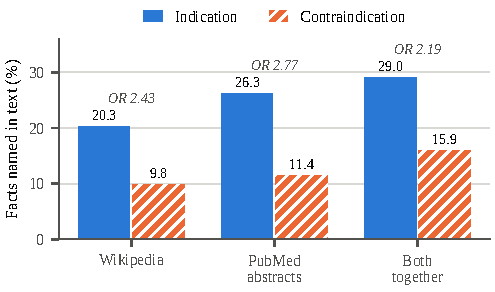
\includegraphics[width=\columnwidth]{fig_coverage.pdf}
\caption{Share of facts whose text names the disease, for the same 574 drugs.
Labels give the within-drug Mantel--Haenszel odds ratio.}
\label{fig:coverage}
\end{figure}

\begin{table}[t]
\centering
\small
\setlength{\tabcolsep}{4pt}
\begin{tabular}{lcccc}
\toprule
Corpus & Ind. & Contra. & OR [95\% CI] & $p$ \\
\midrule
Wikipedia & 20.33 & 9.81 & 2.43 [2.01, 2.94] & $2\times10^{-18}$ \\
PubMed & 26.31 & 11.44 & 2.77 [2.33, 3.28] & $5\times10^{-29}$ \\
Both & 29.04 & 15.91 & 2.19 [1.86, 2.57] & $2\times10^{-20}$ \\
\bottomrule
\end{tabular}
\caption{Percent of facts named in prose and the within-drug odds ratio,
indication against contraindication. 574 drugs, 1,722 edges per relation.}
\label{tab:coverage}
\end{table}

Table~\ref{tab:coverage} and Figure~\ref{fig:coverage} give the main result.
In Wikipedia, 20.33\% of indications are named in the drug's article against
9.81\% of contraindications. Within the same drug, the odds of a benefit fact
being named are 2.43 times those of a safety fact. PubMed abstracts give a gap
of the same size, 2.77, so the asymmetry is not a property of the encyclopedia.
The union of both corpora is the most generous prose baseline available: even
there, the odds ratio is 2.19 (95\% CI 1.86--2.57).

\paragraph{Searching harder does not close the gap.}
A natural objection is that general retrieval favors abstracts about what a
drug treats. The PubMed corpus therefore gives the adverse-effect and
contraindication query its own half of the budget. Over the same 1,722
contraindication edges, coverage was 10.22\% with a single relevance-ranked
query of 40 abstracts and 11.44\% with the split budget, while indication
coverage rose from 23.34\% to 26.31\% under the same change. The within-drug
odds ratio is 2.77 under both retrieval schemes.

\paragraph{The gap concentrates in drugs with few facts.}
Figure~\ref{fig:degree} shows the gap by the drug's number of edges in the
relation. It is 13.94 points for drugs with 3 to 5 edges in Wikipedia, 6.04
for 6 to 12, and 1.64 for 13 or more. The combined corpora show the same
decline (11.81, 6.90, 2.23). In the logistic model, the relation term remains
significant with the edge count held fixed ($p = 2.4\times10^{-4}$ in
Wikipedia, $1.4\times10^{-5}$ in PubMed, $9.7\times10^{-4}$ combined). The gap
is largest for the typical drug, which carries a handful of each.

\paragraph{Some missing evidence is coarser, not absent.}
Relaxing the match shows where the rest of the prose's information sits. On
the draw of 600 edges per relation in Wikipedia, adding synonyms and common
names to the exact name raises coverage by 1.39 points on average across
relations. Adding the disease's MONDO parent raises it by a further 5.50
points, and adding ancestors up to two levels by 8.43. More than four fifths of
the evidence gained by relaxing the match is written at a coarser level than
the graph records, for example ``liver disease'' for a fact about cirrhosis.
Such text is true and relevant, but it does not identify the fact, so we do
not count it as named.

\subsection{The FDA label shows no detectable gap}

\begin{figure}[t]
\centering
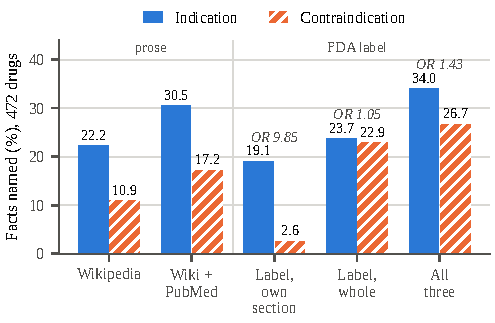
\includegraphics[width=\columnwidth]{fig_label.pdf}
\caption{Share of facts named, on the 472 drugs with an FDA label. ``Own
section'' is Indications and Usage for indications and Contraindications for
contraindications. Labels give the within-drug odds ratio.}
\label{fig:label}
\end{figure}

\begin{table}[t]
\centering
\footnotesize
\setlength{\tabcolsep}{2.2pt}
\begin{tabular}{lcccc}
\toprule
Text & Ind. & Con. & OR [95\% CI] & Deg. \\
\midrule
Wikipedia & 22.25 & 10.95 & & \\
Wiki + PubMed & 30.51 & 17.23 & & \\
Label, own section & 19.07 & 2.61 & 9.85 [7.75, 12.51] & ind.\ \\
Label, whole & 23.73 & 22.88 & 1.05 [0.88, 1.25] & contra.\ \\
All three & 34.04 & 26.69 & 1.43 [1.21, 1.68] & none \\
\bottomrule
\end{tabular}
\caption{Percent of facts named on the same 1,416 edges per relation (472
drugs). ``Deg.'' is the relation favored once the drug's edge count is held
fixed in the logistic model: \emph{ind.}\ and \emph{contra.}\ significant at
$p < 0.01$, \emph{none} $p = 0.86$. Within-drug $p$: $10^{-45}$, 0.62, and
$2\times10^{-5}$.}
\label{tab:label}
\end{table}

If the gap came from the facts themselves, for example because some
contraindications are too rare to write about, it would appear in every source.
It does not. Scored with the same matcher on the same 1,416 edges per relation,
the whole FDA label names 23.73\% of indications and 22.88\% of
contraindications (Figure~\ref{fig:label}, Table~\ref{tab:label}). The
within-drug odds ratio is 1.05 (95\% CI 0.88--1.25, $p = 0.62$). With the
drug's edge count held fixed, the label names contraindications slightly more
often than indications (logistic coefficient $+0.30$, $p = 0.005$), and in no
degree stratum does it favor indications (Figure~\ref{fig:degree}). The
difference in chance floors between the two relations (2.82\% against 2.10\%)
is too small to account for this.

\paragraph{Where in the label.}
The label's own Contraindications section names only 2.61\% of PrimeKG's
contraindications, and for 9.5\% of contraindication edges the section is
empty. The harm facts sit elsewhere in the label: in the Boxed Warning, in
Warnings and Precautions, and in Use in Specific Populations. A retrieval
system that reads only the Contraindications section of a label misses most of
them.

\paragraph{Adding the label to prose.}
Combining all three corpora raises coverage to 34.04\% and 26.69\% and lowers
the odds ratio to 1.43; with edge counts held fixed the relation term is no
longer significant ($p = 0.86$). Of the 1,172 contraindications that neither
Wikipedia nor PubMed names, the label names 11.4\%. The asymmetry is therefore
a property of prose, not of the facts: the record that regulation requires
documents harm as often as benefit, and the text that general-purpose models
read does not.

\begin{figure}[t]
\centering
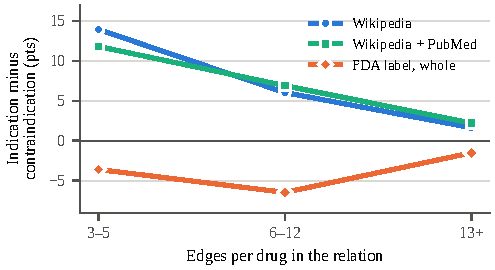
\includegraphics[width=\columnwidth]{fig_degree.pdf}
\caption{Gap between indication and contraindication coverage, by the drug's
number of edges in the relation. Prose favors indications in every stratum;
the whole FDA label does not.}
\label{fig:degree}
\end{figure}

\subsection{Scale buys benefits, not harms}

\begin{figure}[t]
\centering
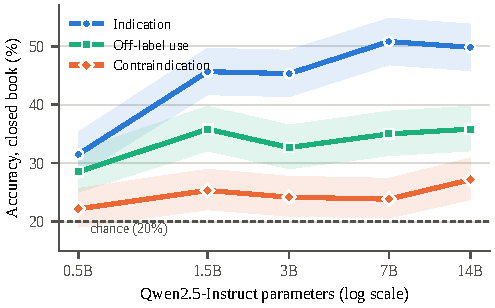
\includegraphics[width=\columnwidth]{fig_scale.pdf}
\caption{Closed-book accuracy on 600 edges per relation, five options, across
five sizes of Qwen2.5-Instruct. Bands are 95\% Wilson intervals.}
\label{fig:scale}
\end{figure}

\begin{table}[t]
\centering
\small
\setlength{\tabcolsep}{2.1pt}
\begin{tabular}{lcccc}
\toprule
Qwen2.5 & Ind. & Off-label & Contra. & Gap [95\% CI] \\
\midrule
0.5B & 31.50 & 28.50 & 22.17 & $+9.3$ [4.0, 14.9] \\
1.5B & 45.67 & 35.83 & 25.33 & $+20.3$ [15.2, 26.2] \\
3B & 45.33 & 32.67 & 24.17 & $+21.2$ [16.1, 26.9] \\
7B & 50.83 & 35.00 & 23.83 & $+27.0$ [21.6, 32.4] \\
14B & 49.83 & 35.83 & 27.17 & $+22.7$ [17.1, 28.3] \\
\midrule
Wikipedia names it & 17.17 & 10.50 & 5.50 & \\
Chance floor & 1.22 & 0.72 & 0.78 & \\
\bottomrule
\end{tabular}
\caption{Closed-book accuracy (\%) on the probe sample, chance 20\%. ``Gap'' is
indication minus contraindication, with a 95\% bootstrap interval over drugs.
The last two rows give the exact-name match in Wikipedia for the same edges and
its chance floor.}
\label{tab:probe}
\end{table}

Figure~\ref{fig:scale} and Table~\ref{tab:probe} show the model side. Across a
28-fold range in parameters, indication accuracy rises from 31.50\% to about
50\%, flattening from 7B. Contraindication accuracy stays between 22.17\% and
27.17\% at every size, within 7 points of chance. The gap opens by 1.5B and
stays between 20 and 27 points through 14B. The paired test between 0.5B and 7B
confirms that scale helps the two relations unequally: the gain on indications
(19.33 points) exceeds the gain on contraindications (1.67 points) by 17.67
points (95\% CI 12.68--22.70, $p = 4.8\times10^{-12}$, 709 drugs resampled).
From 0.5B to 14B, the gains are 18.33 points for indications, 7.33 for
off-label use, and 5.00 for contraindications.

The ordering of accuracy follows the ordering of prose coverage across all
three relations: indications are named most often and answered best,
contraindications are named least often and answered worst, and off-label use
sits between them on both measures. This is the pattern expected when the
training signal for a relation is thin, although our data do not measure the
models' training corpora directly.

\paragraph{The gap holds under harder distractors.}
Table~\ref{tab:distractors} repeats the comparison with wrong options drawn
from the true disease's own neighborhood in MONDO. The gap appears in all four
models and three model families, from 7.9 points in Qwen2.5 0.5B to 45.9 in
Granite 3.1 8B, and it holds within each naming group.

\begin{table}[t]
\centering
\small
\setlength{\tabcolsep}{4.5pt}
\begin{tabular}{lccccc}
\toprule
Model & Ind. & Contra. & Gap & Within & $p$ \\
\midrule
Qwen2.5 0.5B & 36.0 & 28.1 & +7.9 & +8.2 & $0.009$ \\
Qwen2.5 7B & 56.0 & 25.1 & +30.9 & +31.3 & $<10^{-15}$ \\
OLMo 2 7B & 56.0 & 33.0 & +23.0 & +23.6 & $2\times10^{-13}$ \\
Granite 3.1 8B & 58.7 & 12.8 & +45.9 & +46.3 & $<10^{-15}$ \\
\bottomrule
\end{tabular}
\caption{Closed-book accuracy (\%) with distractors from the answer's MONDO
neighborhood plus a ``Not enough information'' option; 450 indication and 406
contraindication questions. ``Within'' is the difference within groups of
questions whose page names the answer, its family, or nothing, which sets the
$p$-value.}
\label{tab:distractors}
\end{table}

\begin{figure}[t]
\centering
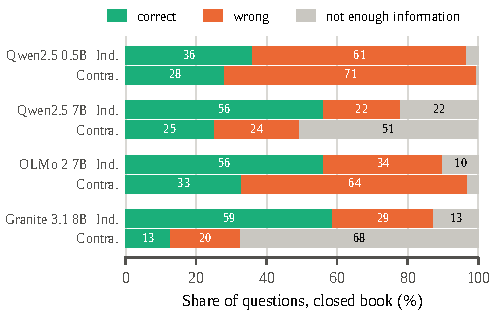
\includegraphics[width=\columnwidth]{fig_failure.pdf}
\caption{Outcome of each closed-book question with harder distractors. On
contraindications, two models mostly guess wrong and two mostly decline.}
\label{fig:failure}
\end{figure}

\paragraph{Two ways of not knowing.}
The ``Not enough information'' option separates two failure styles
(Figure~\ref{fig:failure}, Table~\ref{tab:failure}). Qwen2.5 0.5B and OLMo~2 7B rarely decline and answer
most contraindication questions wrongly (71.4\% and 64.0\% wrong). Qwen2.5 7B
and Granite 3.1 8B decline most of them (50.7\% and 67.5\%) while declining
indications far less (22.0\% and 12.7\%). In every model, precision on the
contraindications it does answer is lower than on indications, by 9 to 28
points. Neither style supplies the fact: one guesses, the other abstains.

\begin{table}[t]
\centering
\footnotesize
\setlength{\tabcolsep}{2.6pt}
\begin{tabular}{lcccccc}
\toprule
 & \multicolumn{3}{c}{Indication} & \multicolumn{3}{c}{Contraindication} \\
\cmidrule(lr){2-4}\cmidrule(lr){5-7}
Model & wrong & decl. & prec. & wrong & decl. & prec. \\
\midrule
Qwen2.5 0.5B & 60.7 & 3.3 & 37.2 & 71.4 & 0.5 & 28.2 \\
Qwen2.5 7B & 22.0 & 22.0 & 71.8 & 24.1 & 50.7 & 51.0 \\
OLMo 2 7B & 34.0 & 10.0 & 62.2 & 64.0 & 3.0 & 34.0 \\
Granite 3.1 8B & 28.7 & 12.7 & 67.2 & 19.7 & 67.5 & 39.4 \\
\bottomrule
\end{tabular}
\caption{How models fail, closed book, harder distractors (\%). ``Decl.'' is
the share answering ``Not enough information''; ``prec.'' is accuracy among
questions the model answered.}
\label{tab:failure}
\end{table}

\subsection{Retrieval helps safety facts when they are written}

\begin{figure}[t]
\centering
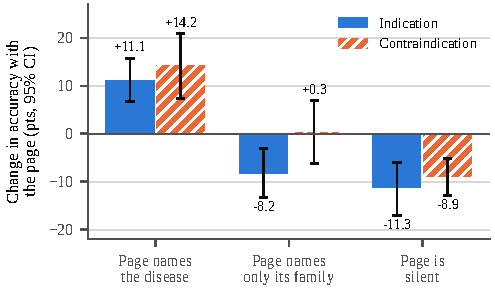
\includegraphics[width=\columnwidth]{fig_retrieval.pdf}
\caption{Change in accuracy when the drug's page is placed in the prompt,
pooled over the three 7--8B models, by what the page says about the answer.}
\label{fig:retrieval}
\end{figure}

\begin{table}[t]
\centering
\footnotesize
\setlength{\tabcolsep}{2.6pt}
\begin{tabular}{lcccccc}
\toprule
 & \multicolumn{2}{c}{Names it} & \multicolumn{2}{c}{Family only} & \multicolumn{2}{c}{Silent} \\
\cmidrule(lr){2-3}\cmidrule(lr){4-5}\cmidrule(lr){6-7}
Model & Ind. & Con. & Ind. & Con. & Ind. & Con. \\
\midrule
Qwen2.5 0.5B & +39.3 & +40.7 & +10.7 & +3.8 & +7.3 & $-6.0$ \\
Qwen2.5 7B & +6.7 & +10.7 & $-12.0$ & $-7.5$ & $-16.7$ & $-14.0$ \\
OLMo 2 7B & +12.7 & +12.7 & $-2.7$ & 0.0 & $-1.3$ & $-5.3$ \\
Granite 3.1 8B & +14.0 & +19.3 & $-10.0$ & +8.5 & $-16.0$ & $-7.3$ \\
\midrule
Pooled 7--8B & +11.1 & +14.2 & $-8.2$ & +0.3 & $-11.3$ & $-8.9$ \\
\bottomrule
\end{tabular}
\caption{Change in accuracy (points) from closed book to the drug's page, by
what the page says about the answer. 150 questions per cell, except 106
family-only contraindication questions.}
\label{tab:retrieval}
\end{table}

If models failed on contraindications because they could not use safety
information, giving them the page would help indications more. It does not.
When the page names the disease, the passage raises accuracy by 11.1 points on
indications and 14.2 points on contraindications, pooled over the three 7--8B
models (Figure~\ref{fig:retrieval}, Table~\ref{tab:retrieval}). The difference,
$-3.1$ points (95\% CI $-11.6$ to $+5.1$), is not significant, and the pattern
holds in each model.

When the page is silent, accuracy falls with the page for both relations, by
11.3 and 8.9 points. The loss comes from declines: with a silent page, Qwen2.5
7B answers ``Not enough information'' on 94.0\% of contraindication questions
against 56.0\% closed book, and Granite on 92.7\% against 71.3\%. That is the
right response to a page that does not contain the answer.
Pooled over the three 7--8B models (table in the supplement), the shift is the same. Declines rise most with a silent page (by 32.9 points on
contraindications and 26.0 on indications), less with a page that names only
the family (12.3 and 16.9), and barely with a page that names the answer (5.4
and $-0.2$).


Retrieval therefore
helps safety facts about as much as benefit facts; we detect no difference. What differs is
how often there is anything to retrieve: in prose, 17\% of contraindications
against 30\% of indications on the label sample.

\subsection{The control graph shows no gap}

On Hetionet, Wikipedia names the disease for 57.33\% of \emph{treats} edges and
56.10\% of \emph{palliates} edges (odds ratio 1.05, $p = 0.70$), against a
within-drug odds ratio of 2.43 between indications and contraindications in
PrimeKG on the same corpus. Within the 51 drugs that carry both Hetionet
relations, \emph{treats} edges are named more often (odds ratio 2.48, 95\% CI
1.29--4.75), but this difference disappears once the drug's edge count is held
fixed: the relation term in the logistic model has $p = 0.16$, and the degree
strata show no consistent direction. The PrimeKG gap survives the same control.
Together with the FDA label, which shows no gap under the same matcher, the
control shows that the measurement does not produce a gap where the sources do
not have one.



\subsection{Summary of checks}

Table~\ref{tab:checks} lists the alternative explanations we tested and the
result of each. Each explanation that would make the prose gap an artifact of
the drugs, the corpora, the retrieval, the matcher, or the models is addressed
by at least one test, and the FDA label argues against an explanation in terms
of the facts themselves.

\begin{table}[t]
\centering
\footnotesize
\setlength{\tabcolsep}{2.5pt}
\begin{tabular}{p{2.55cm}p{2.6cm}p{2.45cm}}
\toprule
Explanation & Test & Result \\
\midrule
Famous drugs dominate & Within-drug MH odds ratio & 2.19--2.77 in prose \\
Many contraindications per drug & Logistic model, degree strata & Gap holds, $p \le 10^{-3}$ \\
One editorial process & Wikipedia and PubMed separately & 2.43 and 2.77 \\
Retrieval favors efficacy & Split PubMed budget & OR 2.77 both ways \\
Matcher favors a relation & Hetionet, two benefit relations & No gap, $p = 0.16$ \\
Coincidental matches & Floor on unrelated diseases & $\le$ 1.2\% prose, $\le$ 2.8\% label \\
Facts are too rare to write & Whole FDA label & OR 1.05, $p = 0.62$ \\
Small models only & Five sizes, 0.5B--14B & Contra.\ within 7 pts of chance \\
Easy distractors & MONDO siblings, 4 models & Gap 7.9--45.9 pts \\
Models cannot use safety text & Page in the prompt & $+14.2$ vs.\ $+11.1$ pts \\
\bottomrule
\end{tabular}
\caption{Alternative explanations for the gap and the tests that address them.}
\label{tab:checks}
\end{table}

\section{Discussion}

\begin{figure*}[t]
\centering
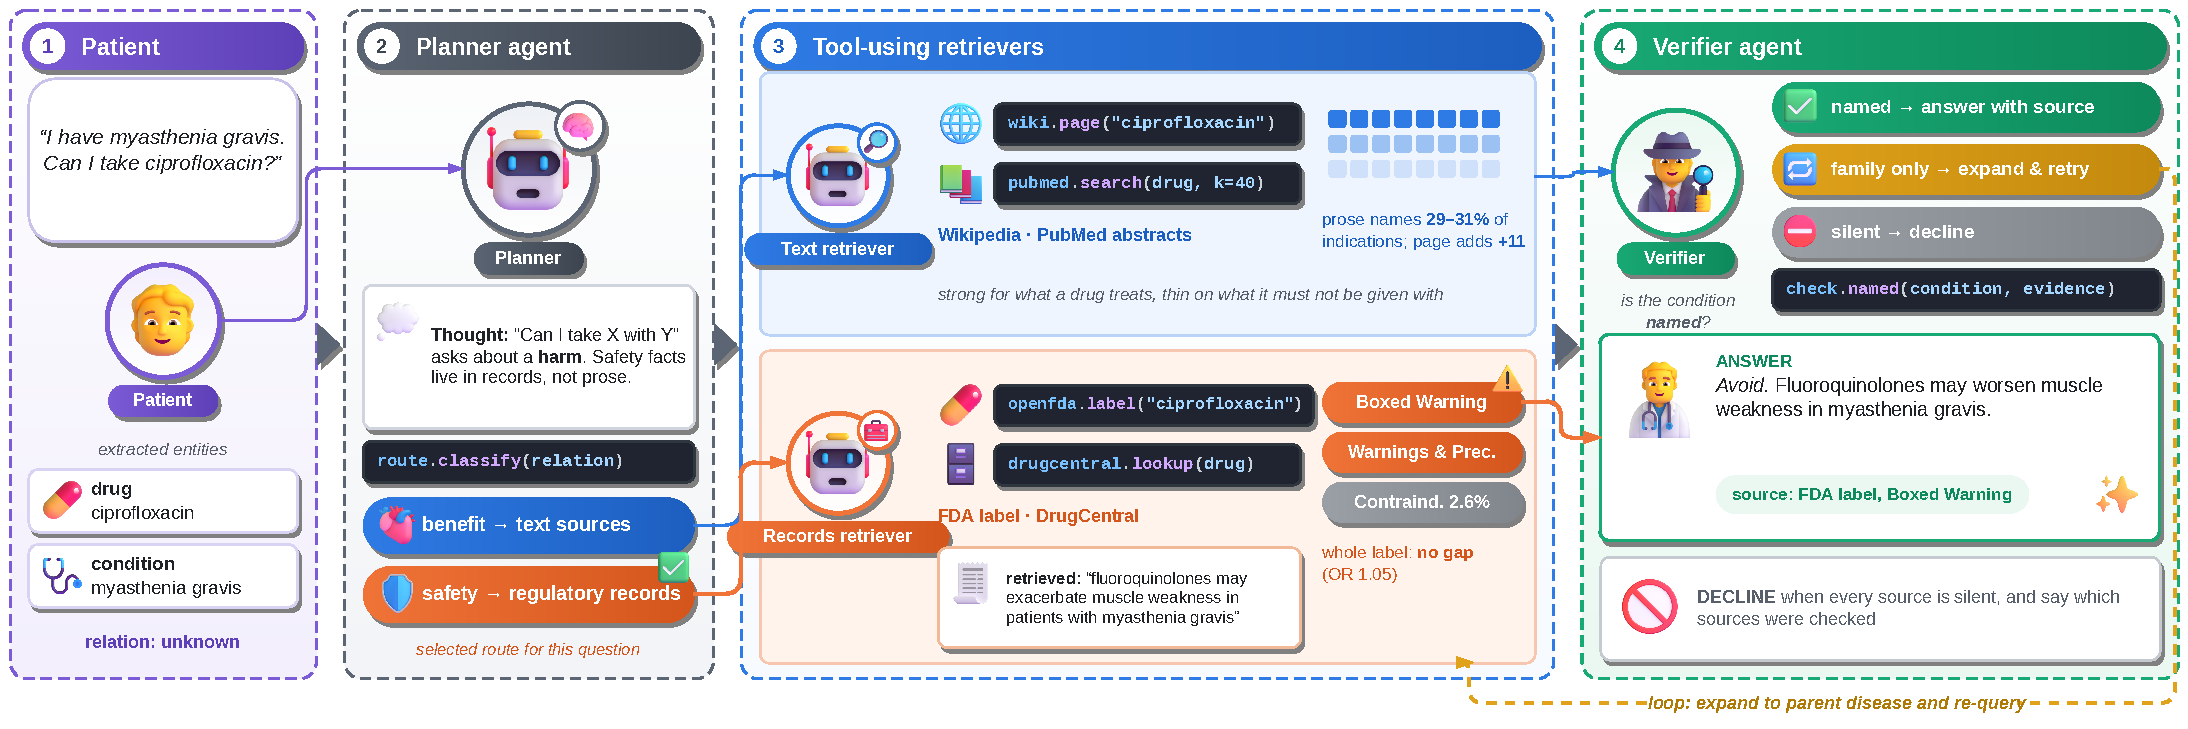
\includegraphics[width=\textwidth]{fig_router.pdf}
\caption{A relation-aware routing design for clinical agents that follows from
the measurements. A controller classifies the question as benefit or safety and
chooses the retrieval route; a checker decides between answering with a cited
source, expanding a family-level mention, and declining with the name of the
silent source. The example answer paraphrases the Boxed Warning of the
ciprofloxacin label.}
\label{fig:router}
\end{figure*}

\paragraph{Safety is the blind spot of prose.}
Across two prose corpora that share no editorial process, the facts that
matter most for harm are the ones least often written down. The label, which
regulation requires to carry them, shows no such gap. One explanation is that
prose is organized around what a drug is for: the encyclopedia for a general
reader, the literature around efficacy. Even abstracts retrieved for toxicity
rarely name the specific condition that forbids a drug.

\paragraph{Scale did not fix it.}
If contraindication errors came from limited capacity, scale would reduce
them. Across five sizes, the gain goes almost entirely to indications and
contraindication accuracy stays near chance. Larger models also change how
they fail rather than whether they know: the 7--8B models in
Table~\ref{tab:failure} either guess or decline on most safety questions.

\paragraph{What this means for clinical agents.}
The special theme of this year's workshop is agentic biomedical and clinical
workflows. An agent that answers a medication question by reading prose, or by
consulting its own weights, is exposed to the asymmetry measured here.
Figure~\ref{fig:router} shows a design motivated by the measurements; it is a
proposal, not an evaluated clinical system. A
controller first classifies the question by relation. Benefit questions can
be answered from prose with an evidence check, since prose names 29--31\% of
indications and the page helps when it does. Safety questions go to a
structured source such as DrugCentral and to the whole FDA label, not only its
Contraindications section, which names 2.6\% of PrimeKG's contraindications.
An evidence check then decides between answering with the matched sentence and
declining with the name of the source that was silent. The per-fact matcher
used here is cheap enough to serve as that check.

\paragraph{What this means for retrieval design.}
Three practical rules follow. First, the corpus matters by relation: adding the
label to prose closes most of the safety gap (odds ratio 2.19 to 1.43), while
adding more prose of the same kind does not (2.43 to 2.19). Second, the
section matters: a label retriever that indexes only the Contraindications
section sees 2.6\% of the safety facts that the whole label names 22.9\% of.
Third, much of what prose does say about a disease is said at the level of its
family, and such a passage is relevant without being sufficient; a system
should treat it as a reason to look further, not as an answer.

\paragraph{Off-label use sits in between.}
Off-label uses are benefit facts that a drug's label does not approve. They are
named in prose less often than indications and more often than
contraindications, and model accuracy and its gain from scale fall in the same
middle position. Across the three relations, the ordering of model accuracy
follows how often text names them, not whether they describe benefit or harm.

\paragraph{What this means for evaluation.}
Medical benchmarks usually report one accuracy per model. Our results show that
the average hides a relation that sits near chance and does not improve with
scale. Benchmarks built from knowledge graphs should report accuracy per
relation, and in particular for contraindications, so that gains on benefit
facts are not read as gains in safety.

\paragraph{An example.}
A patient with myasthenia gravis asks whether an antibiotic is safe for them.
PrimeKG records that ciprofloxacin is contraindicated in this disease. Across
our sample, a contraindication of this kind is named in its drug's Wikipedia
article about one time in ten, a 7B model picks it out of five options about
one time in four, and the label, read in full, names safety facts as often as
benefit facts.

\section{Limitations}

\paragraph{Corpus to model.} The link from corpus to model is correlational:
we measure public corpora, not the models' training data. Two prose corpora
with the asymmetry, a label without it, and models that follow the prose make
the link plausible, but the causal chain is not demonstrated. PubMed figures
come from abstracts and are a lower bound.

\paragraph{Matching.} String matching misses paraphrases and can match a name
used in an unrelated sense; the floor bounds the second error at under 3\%. A
name match also does not show that the text asserts the relation, which a
blinded audit of matched sentences would measure. Both errors apply to both
relations on the same text.

\paragraph{Models and questions.} The scale curve uses one model family; the
distractor and page tests add two more at one size each. Multiple choice
measures recognition rather than recall.

\paragraph{Graph labels.} Even the whole label names only about a quarter of
PrimeKG's sampled contraindications, so many edges are recorded more
specifically than any text states them. A clinical review of unnamed
contraindications would separate specificity from omission.

\section{Ethical Considerations}

The study uses only public graphs, text and drug labels, and no patient data.
Its results are not guidance on any individual drug: a fact's absence from
prose does not make it uncertain, and the contraindications studied here remain
authoritative in the sources that record them. Code that rebuilds every number
is released with the paper.

\section{Conclusion}

The \lbl{} asymmetry is specific to prose: text names a drug's efficacy about
twice as often as its limits, and the FDA label does not. Medication-safety
questions should be routed to the label.

\bibliography{refs}

\end{document}
